\chapter{Active Directory Attacks-Steps, Types, and Signatures}

\chapter{Active Directory Attacks—Steps, Types, and Signatures}

\section{Introduction}

The Microsoft domain environment is one of the most critical components of modern enterprise networks. The core of this environment is \textbf{Active Directory (AD)}—Microsoft’s implementation of directory services—providing essential functions such as user and identity management, authentication, and centralized policy enforcement. As the most widely adopted directory service in the Windows ecosystem, AD plays a fundamental role in enabling secure access and resource management within organizations.

Active Directory offers several integrated services, including:

\begin{itemize}
    \item \textbf{Domain Services (AD DS):} Enable communication between users and domains, manage centralized data storage, and support login and search operations.
    \item \textbf{Certificate Services:} Issue, manage, and distribute digital certificates for authentication and encryption.
    \item \textbf{Lightweight Directory Services (AD LDS):} Provide support for directory-enabled applications using the Lightweight Directory Access Protocol (LDAP).
    \item \textbf{Federation Services (AD FS):} Facilitate single sign-on (SSO) across multiple web applications and services.
    \item \textbf{Rights Management Services (RMS):} Protect digital content by enforcing usage policies and preventing unauthorized distribution.
    \item \textbf{DNS Services:} Handle domain name resolution for AD-integrated systems.
\end{itemize}

Due to its central role in managing authentication and access to nearly all enterprise resources, Active Directory is vital not only for system administrators and defenders but also for offensive security teams. Its widespread use and elevated privileges make it a prime target for cyber attackers—especially those deploying \textbf{Advanced Persistent Threats (APTs)}.

The United States Air Force (USAF) defines APTs based on three core attributes:

\begin{itemize}
    \item \textbf{Advanced:} Adversaries possess deep knowledge of intrusion tools and tactics and can develop custom exploits.
    \item \textbf{Persistent:} The attacker operates with long-term mission focus and sustained access.
    \item \textbf{Threat:} The actors are organized, well-funded, and highly motivated—often linked to nation-state operations.
\end{itemize}

\renewcommand{\arraystretch}{1.4}
\begin{longtable}{|p{4cm}|p{11cm}|}
\caption{Advanced Persistent Threats (APT): Characteristics and Detection Measures} \\
\hline
\rowcolor{gray!20} \textbf{Attribute} & \textbf{Description} \\
\hline
\endfirsthead

\multicolumn{2}{c}{{\bfseries Table continued}} \\
\hline
\rowcolor{gray!20} \textbf{Attribute} & \textbf{Description} \\
\hline
\endhead

\hline \multicolumn{2}{r}{{Continued on next page}} \\
\endfoot

\hline
\endlastfoot

\textbf{Nomenclature Meaning} & \textbf{Advanced:} The adversary has deep knowledge of intrusion tools and can develop custom exploits. \newline
\textbf{Persistent:} The attacker maintains long-term access and returns repeatedly. \newline
\textbf{Threat:} The attacker is organized, well-funded, and strategic. \\
\hline

\textbf{Common Signs} & Nation-state groups (e.g., APT28, Deep Panda), extended access, sophisticated techniques, low detection risk, high-value targets. \\
\hline

\textbf{Lifecycle} & Reconnaissance → Initial Compromise → Establish Foothold → Privilege Escalation → Lateral Movement → Maintain Access → Data Exfiltration. \\
\hline

\textbf{Techniques} & Social engineering, spear phishing, watering hole attacks, credential theft, drive-by downloads, and custom malware. \\
\hline

\textbf{Target Sectors} & Government, IT, finance, energy, healthcare, logistics, manufacturing. \\
\hline

\textbf{Comparison with Malware} & APTs are strategic and long-term; traditional malware is opportunistic. APTs aim for espionage; malware often aims for profit. \\
\hline

\textbf{Defense Measures} & Email filtering, EDR, MFA, access controls, user and network monitoring, behavioral analytics. \\
\hline
\end{longtable}

\textbf{Note:} The above table helps contextualize APTs by comparing them with traditional malware and highlighting detection strategies.

\bigskip

\textbf{Objective of This Chapter:}
\begin{itemize}
    \item Describe the typical AD attack lifecycle and mitigation strategies.
    \item Present observable attack signatures for Kerberoasting and Pass-the-Hash attacks.
    \item Analyze how Kerberos protocol is exploited in privilege escalation.
    \item Explore how attackers use social engineering and human behavioral weaknesses.
\end{itemize}

\section{Background: Kerberos and AD Security}

This section introduces the Kerberos protocol, focusing on its authentication workflow, concepts, and security weaknesses in AD environments.

\subsection{Kerberos Authentication Workflow}

Kerberos is the default authentication protocol in Active Directory. It facilitates mutual authentication between clients and services using a trusted third-party—the \textit{Key Distribution Center (KDC)}.

The KDC operates on Domain Controllers and consists of:
\begin{itemize}
    \item \textbf{Authentication Server (AS):} Verifies identity and issues a Ticket Granting Ticket (TGT).
    \item \textbf{Ticket Granting Service (TGS):} Issues service-specific tickets after verifying a valid TGT.
\end{itemize}

When a user logs in, this process occurs:
\begin{enumerate}
    \item User sends encrypted timestamp to AS.
    \item AS validates it and returns:
        \begin{itemize}
            \item Session key encrypted with user password hash.
            \item TGT encrypted with the krbtgt account's key.
        \end{itemize}
    \item User sends TGT to TGS with an authenticator.
    \item TGS responds with:
        \begin{itemize}
            \item Service ticket encrypted with the service's key.
            \item Session key for use between client and target server.
        \end{itemize}
    \item Client sends service ticket to target server, which authenticates the user.
\end{enumerate}

This provides mutual authentication—but if the krbtgt account is compromised, attackers can forge tickets ("Golden Ticket" attack).

\subsection{Kerberos Security Issues}

Two major risks exist:
\begin{enumerate}
    \item The \texttt{krbtgt} password is rarely changed and never expires.
    \item If stolen, attackers can forge tickets that bypass most detection methods.
\end{enumerate}

\textbf{\chapter{Active Directory Attacks—Steps, Types, and Signatures}

\section{Introduction}

The Microsoft domain environment is one of the most critical components of modern enterprise networks. The core of this environment is \textbf{Active Directory (AD)}—Microsoft’s implementation of directory services—providing essential functions such as user and identity management, authentication, and centralized policy enforcement. As the most widely adopted directory service in the Windows ecosystem, AD plays a fundamental role in enabling secure access and resource management within organizations.

Active Directory offers several integrated services, including:

\begin{itemize}
    \item \textbf{Domain Services (AD DS):} Manage centralized data storage, support login and search operations.
    \item \textbf{Certificate Services:} Issue and manage digital certificates for authentication/encryption.
    \item \textbf{Lightweight Directory Services (AD LDS):} Supports directory-enabled applications using LDAP.
    \item \textbf{Federation Services (AD FS):} Enables single sign-on (SSO) across web applications/services.
    \item \textbf{Rights Management Services (RMS):} Enforce content usage policies and protect digital documents.
    \item \textbf{DNS Services:} Provide name resolution for AD-integrated systems.
\end{itemize}

Due to its central role in authentication and access, AD is critical not only for defenders but also for attackers. Its privileges and widespread use make it a prime target—especially by \textbf{Advanced Persistent Threats (APTs)}.

The USAF defines APTs with three core traits:
\begin{itemize}
    \item \textbf{Advanced:} Skilled adversaries capable of custom exploit development.
    \item \textbf{Persistent:} Long-term, mission-focused campaigns with sustained access.
    \item \textbf{Threat:} Organized, well-funded, highly motivated—often state-sponsored.
\end{itemize}

\vspace{1em}
\renewcommand{\arraystretch}{1.4}
\begin{longtable}{|p{4cm}|p{11cm}|}
\caption{APT Characteristics and Detection Measures} \\
\hline
\rowcolor{gray!20} \textbf{Attribute} & \textbf{Main Features and Description} \\
\hline
\endfirsthead

\hline \multicolumn{2}{r}{{Continued on next page}} \\
\endfoot

\hline
\endlastfoot

\textbf{Nomenclature Meaning} &
\textbf{Advanced:} Adversaries have deep technical expertise and can craft custom malware. \newline
\textbf{Persistent:} Long-term operations with sustained infrastructure. \newline
\textbf{Threat:} Well-organized, often linked to nation-states. \\
\hline

\textbf{Signs} &
Actors include APT28, OilRig, Deep Panda. Goals involve espionage and disruption. Use rootkits, DNS tunneling, rogue Wi-Fi. Often stealthy and cautious. \\
\hline

\textbf{Lifecycle} &
\textbf{1. Initial Reconnaissance:} Identify systems and users. \newline
\textbf{2. Initial Compromise:} Deploy malware, gain initial access. \newline
\textbf{3. Establish Foothold:} Maintain persistent access. \newline
\textbf{4. Escalate Privileges:} Use tools like mimikatz or token theft. \newline
\textbf{5. Internal Recon:} Map network, locate assets. \newline
\textbf{6. Lateral Movement:} Jump between hosts. \newline
\textbf{7. Maintain Presence:} Create persistence mechanisms. \newline
\textbf{8. Complete Mission:} Exfiltrate data, disrupt operations. \\
\hline

\textbf{Techniques} &
Social engineering, spear-phishing, watering hole attacks, drive-by downloads. Often tailored to the target. \\
\hline

\textbf{Targets} &
\textbf{Government:} Surveillance, disruption. \newline
\textbf{Finance:} Steal data, money. \newline
\textbf{Healthcare:} Leak medical records. \newline
\textbf{Energy/Utilities:} Sabotage. \newline
\textbf{IT Sector:} IP theft. \newline
\textbf{Transport:} Disruption. \newline
\textbf{Manufacturing:} Industrial espionage. \\
\hline

\textbf{Malware Comparison} &
\textbf{APTs:} Long-term, stealthy, strategic. \newline
\textbf{Typical Malware:} Broad, opportunistic, often short-lived. \newline
\textbf{APTs:} May use malware as just one part of a broader strategy. \\
\hline

\textbf{Detection and Defense} &
Email filtering, endpoint detection and response (EDR), strict access controls, traffic monitoring, user behavior analytics. \\
\hline
\end{longtable}

Most cyberattacks in enterprise environments begin by compromising a single workstation. From there, attackers escalate their access, typically aiming to compromise high-privileged accounts-especially domain administrators-who possess unrestricted access to nearly all resources within the organization. To maintain presence, attackers often deploy various persistence techniques, ensuring continued access at an elevated privilege level for as long as possible.

As businesses increasingly adopt digital platforms and services, securing organizational infrastructure against cyber threats becomes critical. According to a report by Kaspersky, the average cost of a data breach is approximately \$1.41 million for companies and \$108,000 for small and medium companies. These statistics underscore the growing concern around Active Directory (AD) security and have driven significant research into attach techniques and defensive mechanisms related to AD environments.

This chapter focuses on \textit{privilege escalation techniques} used in Active Directory attacks. We also discuss a variety of mitigation strategies that aim to detect, minimize, and prevent such attacks. Additionally, two other attacks of interest that we will be covering include the Pass-the-Hash (PtH) and Kerberoasting attacks.

The key objectives of this chapter are as follows.
\begin{itemize}
    \item Summarize the main characterizing attributes of Advanced Persistent Threats (APTs), including their definitions, signs, lifecycle stages, techniques, target types, comparison with malware, and associated detection and protection strategies.
    \item Describe the typical attack lifecycle within Active Directory environments and describe the methods used at each stage.
    \item Present the attack signatures for both Pass-the-Hash (PtH) and Kerberoasting attacks.
    \item Analyze how the Kerberos authentication protocol is exploited in different stages of an AD attack lifecycle.
\end{itemize}

\subsection{Chapter Organization}
\begin{itemize}
    \item Section 2 provides background on the Kerberos authentication mechanism, a core component of Active Directory, and a common target in AD-based attacks.
    \item Section 3 presents the attack lifecycle that is typically observed in AD environments.
    \item Section 4 reviews the existing work related to Active Directory defense and mitigation strategies.
    \item Section 5 details the finding on privilege-escalation attacks in AD.
    \item Section 6 concludes the chapter and describes best practices for attack prevention.
\end{itemize}

\section{Background}
This section provides essential background information on the Kerberos authentication protocol, focusing on its operational workflow and associated security challenges. Kerberos plays a central role in the security of Active Directory (AD) environments, and a deep understanding of its mechanisms is fundamental to the analysis of AD-related attacks.

\subsubsection{Kerberos Authentication Workflow}
Kerberos is the default authentication protocol used in Active Directory environments. Facilitates mutual authentication between clients and services, ensuring secure access to network resources. Entities that participate in authentication and resource access using Kerberos are referred to as \textit{principals.}

The core of the protocol is the \textit{Key Distribution Center (KDC),}, which handles both authentication and ticket issuance. The KDC operates on any writable Domain Controller (DC) and consists of two main components:
1. Authentication Server (AS): Verifies the identity of the client and issues a \textit{Ticket Granting Ticket (TGT).}
2. Ticket Granting Service (TGS): Issues service-specific tickets to authenticated users holding a valid TGT.

Understanding the Kerberos workflow is critical to analyzing attacks on Active Directory, as many attack vectors-including Pass-the-Hash (PtH) and Kerberoasting-leverage vulnerabilities or design aspects of this protocol.

When a user or service requests access to a protected resource within an AD environment, the Kerberos authentication process follows a structured sequence of steps. This process is summarized in Figure 1.

\begin{figure}
    \centering
    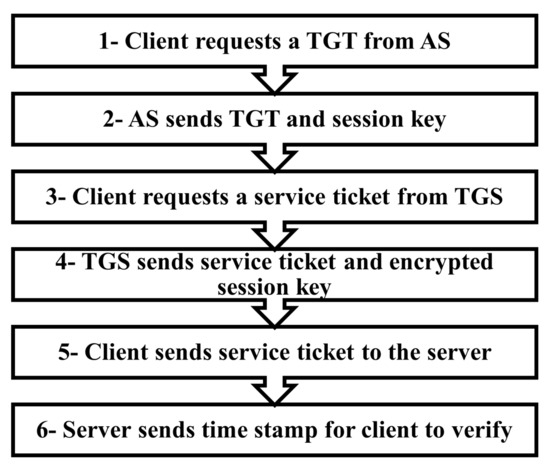
\includegraphics[width=1\linewidth]{tgtflow.png}
    \caption{\textbf{FIGURE 1. }Kerberos Authentication Workflow}
    \label{fig:placeholder}
\end{figure}

\subsubsection{Kerberos Authentication Concepts}
Kerberos uses \textit{symmetric key cryptography} and a trusted third-party-the \textit{Key Distribution Center (KDC)}-to authenticate clients and grant access to services within an Active Directory environment. The process involves multiple exchanges between the client and \textit{ authentication server (AS),} the \textit{ ticket grant service (TGS),} and the target service. The complete workflow is described as follows:

\textbf{1. Password Hashing:}
\begin{itemize}
    \item The client generates a hash of the user password, which serves as a \textit{secret key} for securing communications within the KDC.
\end{itemize}
\textbf{2. Authentication Request to AS:}
\begin{itemize}
    \item The client sends an encrypted timestamp, secured with the hashed password, to the AS. The AS then verifies the client's identity by attempting to decrypt the timestamp using the corresponding password hash stored in the Active Directory database, \texttt{ntds.dit}.
    \begin{itemize}
        \item If decryption is successful, the AS confirms that the client possesses the correct password and allows the user to move forward.
\end{itemize}
    \end{itemize}
\textbf{3. AS Reply (Initial Credentials:}
    The AS responds with two main components: \textbf{(a) A session key,} encrypted with the client password hash, to be used for subsequent communications with the KDC.
            \textbf{(b) A Ticket Granting Ticket (TGT),} which contains the user's identity and metadata. This TGT is encrypted using the krbtgt account's secret key, known only to the TGS. The client stores this TGT and presents it when requesting access to specific services.
\textbf{4. Service Request to TGS:}
To access a specific service, the client sends a request to TGS. This request includes:
the TGT obtained from the AS.
            (a) An \textit{authenticator}, encrypted with the session key, proving the client's identity and the request's validity.
\textbf{5. TGS Response (Service Ticket):}
After successful validation of the TGT and the authenticator, the TGS responds with: \textbf{(a) A service ticket,} encrypted with the secret key of the target service. This ticket includes the user's group membership, a session key for client-server communications, and a timestamp.
            \textbf{(b) The session key,} encrypted with the client's session key (received from the AS), which the client will use to securely communicate with the target service.
\textbf{6. Service Request to the Target Server:}
    Finally, the client sends a request to the target server, including the service ticket obtained from the TGS.
            The server decrypts the ticket using its own key (shared with the KDC).
            If successful, the server confirms that the request is legitimate and that the client has been authenticated by the KDC.

This workflow ensures mutual authentication and secure access control within the AD environment; however, certain aspects of this process-particularly the handling of password hashes and tickets-are susceptible to exploitation, as demonstrated in various AD attacks such as Pass-the-Hash and Kerberoasting.

\subsection{Kerberos Security Issues}
One of the most defining characteristics of the Kerberos protocol is its stateless nature. In this context, "stateless" means that the Key Distribution Center (KDC)-comprising the Authentication Server (AS) and the Ticket Granting Service (TGS)-does not maintain session information for individual clients. Instead, all necessary information to process future service requests is encapsulated within the Ticket Granting Ticket (TGT) itself.

The TGT is encrypted using the secret key of the \texttt{krbtgt} account, which is known only to the components of the KDC-the AS (which issues the TGT) and the TGS (which consumes it to issue service tickets). Because of this encryption model, two important security implications arise:

1. The \texttt{krbtgt} account password is one of the most critical secrets in the Active Directory environment.
2. All information contained within the TGT is inherently trusted by the TGS, since it is assumed that only the AS (a trusted component) could have issued it using the \texttt{krbtgt} key.

A notable security concern is that the password to the \texttt{krbtgt} account is rarely changed. In many environments, never expires and remains static for extended periods. This poses a significant risk: If an attacker manages to compromise the krbtgt password (e.g., through a Golden Ticket attack), they can forge valid TGTs and maintain long-term, stealthy access to the environment. The system remains vulnerable until the \texttt{krbtgt} password is manually rotated-a nontrivial process in most enterprise domains.

\section{Active Directory Attack Phases}
Attacks targeting Active Directory (AD) environments typically follow a structured and sequential lifecycle, progressing through multiple stages. Most reach efforts in this domain focus on post-exploitation scenarios, assuming that an attacker has already established an initial toehold in the environment. This chapter adopts the same perspective, analyzing attack techniques that follow the initial compromise.

Once access to a single user account or machine is gained, the attacker begins by enumerating the domain to collect critical information. This may include domain users, group memberships, trust relationships, and security policies-information necessary for lateral movement and privilege escalation.

The next phase involves privilege hunting, where the adversary actively seeks accounts with elevated privileges, such as local administrators or domain administrators. Upon successful escalating privileges, the attacker shifts focus to persistence, employing techniques to maintain long-term access to the environment. These techniques ensure the attacker can continue operations without needing to re-exploit initial vulnerabilities.

Ultimately, the adversary aims to achieve specific objectives such as data exfiltration, denial of service, sabotage, or ongoing environmental surveillance.

The major phases of a typical AD attack lifecycle are summarized in Figure 2.

\begin{figure}
    \centering
    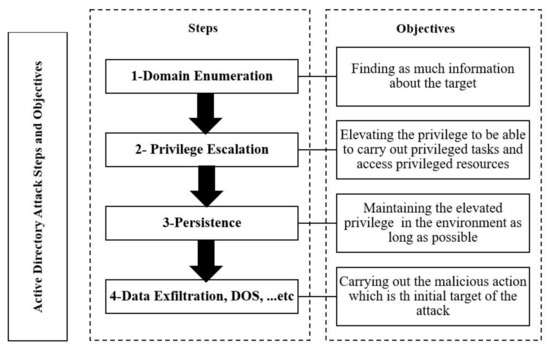
\includegraphics[width=0.75\linewidth]{attacksteps.png}
    \caption{\textbf{FIGURE 2. }Active Directory attack steps}
    \label{fig:placeholder}
\end{figure}

\subsection{Domain Enumeration}
After obtaining an initial toehold within an Active Directory (AD) environment, an attacker's primary objective is typically to escalate privileges-ideally by compromising highly privileged accounts such as Domain Admins or Enterprise Admins. To achieve this, the attacker must first perform a domain enumeration to identify weaknesses or misconfigurations that can be exploited.

In particular, many domain reconnaissance operations can be executed using a standard user account without the need for elevated privileges. Attackers exploit this to gather extensive information about the AD infrastructure, user privileges, group memberships, access control configurations, and active sessions. In this phase a wide range of tools are used, both native to Windows and developed by the security community. The following provides an overview of four commonly used enumeration tools.

\textbf{1. \texttt{net.exe}}
\texttt{net.exe} is a built-in Windows utility used to manage users, groups, network shares, and more. Attackers use it to:
Enumerate all domain users and groups
Identify privileged groups such as Domain Admins
Extract group membership details for specific users

\textbf{2. Active Directory PowerShell Module}
The Active Directory module for PowerShell provides a set of cmdlets that allow administrators to query and manage AD objects. Although this module typically requires Remote Server Administration Tools (RSAT) to be installed, attackers can find ways to import it onto any compromised workstation.

Capabilities include:

Querying domain objects and relationships
Retrieving information about users, computers, groups, and trust relationships

\textbf{3. PowerView}
PowerView is a PowerShell-based tool that is part of the PowerSploit framework. It is designed specifically for domain enumeration and can replicate much of the functionality provided by the AD module.

PowerView extends standard capabilities by enabling:

Identification of where specific users are logged in
Enumeration of group memberships, ACLs, and session information
Discovery of privilege escalation pathways and lateral movement opportunities

\textbf{4. BloodHound}
BloodHound is a graph-based enumeration tool widely used by both red and blue teams to analyze complex AD environments. It collects and visualizes data about user and group relationships, permissions, and attack pathways within a domain.

Key features include:

Mapping of privilege escalation chains
Visualization of effective permissions and attack pathways 
Identification of high-value targets and vulnerable access relationships

The output from domain reconnaissance can be extensive, depending on the time and effort invested in this phase. Common data collected by attackers includes:

Current domain and forest information
List of privileged groups (e.g., Domain Admins, Enterprise Admins)
Noteworthy Access Control List (ACL) entries
Domain structure and Group Policy Objects (GPOs)
Shared resources and sensitive files
Machines where targeted users have active sessions

This comprehensive mapping of the AD environment sets the foundation for subsequent stages such as privilege escalation, lateral movement, and persistence.

\section{Attack Demonstration Using Common Active Directory Enumeration Tools}
The below tools demonstrate how attackers use common Active Directory enumeration tools to support actions such as:

Initial Access / Reconnaissance
Privilege Escalation
Lateral Movement

Below is a breakdown of each tool with sample commands categorized by attacker goals. These examples are for educational and defensive purposes only, as they simulate attacker behavior to help blue teams and defenders detect and mitigate these activities.

\subsection{1. Initial Access / Recon}
\subsubsection{\texttt{net.exe}-Native Windows Tool}

\mybox{cmd}{gray!20}{gray!40}{\texttt{net user /domain}}
Lists all domain users. Can reveal naming conventions, target users.

\mybox{cmd}{gray!20}{gray!40}{\texttt{net group "Domain Admins" /domain}}
Enumerates members of the \texttt{Domain Admins} group.

\mybox{cmd}{gray!20}{gray!40}{\texttt{net view /domain}}
Lists available domains in the environment.

\mybox{cmd}{gray!20}{gray!40}{\texttt{net view \textbackslash\textbackslash<hostname>}}
Lists shared resources on a specific host.

\subsection{2. Privilege Escalation}
\mybox{cmd}{gray!20}{gray!40}{\texttt{net localgroup administrators \textbackslash\textbackslash<target-host>}}
Checks if the current user is in the local \texttt{Administrators} group on a remote host.
\begin{itemize}
    \item \textbf{Advanced:} Attackers have a deep understanding of offensive tools and techniques and can develop custom exploits.
    \item \textbf{Persistent:} The adversary maintains long-term access to systems, executing planned missions, and targeting specific objectives.
    \item \textbf{Threat:} The actor is organized, well funded and highly motivated to compromise strategic assets.
\end{itemize}
Table 1 provides a comprehensive overview of the characteristics of APT, including the meaning behind the nomenclature [5], common indicators or signatures [6], life cycle phases [7], associated techniques [8], comparison of targets and malware types [5][8], and recommended detection and mitigation strategies.

 
In recent years, several high-profile breaches have demonstrated how attackers exploit the human element in cybersecurity. Despite advances in technical safeguards, people remain a critical and vulnerable link in the security chain. Figure 1 illustrates common tools and the general flow of cyberattacks based on social engineering.

\begin{figure}
    \centering
    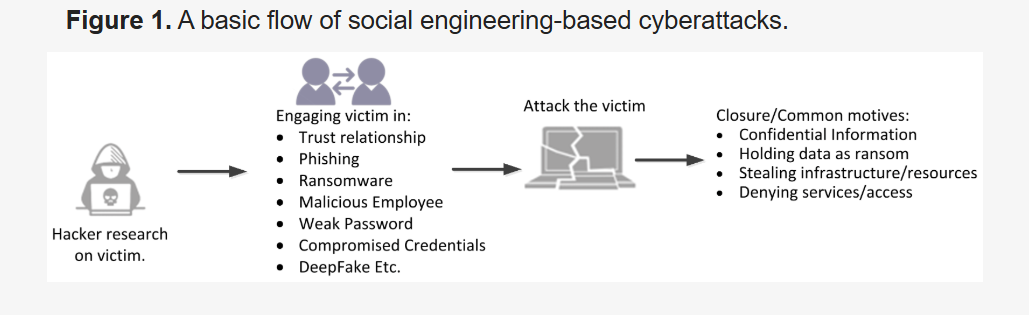
\includegraphics[width=1\linewidth]{soceng.png}
    \caption{Enter Caption}
    \label{fig:placeholder}
\end{figure}
In the past two years, the most common mediums for conducting social engineering (SE) attacks have been through the use of social media platforms and \textit{smishing}(SMS-based phishing) campaigns. The majority of SE attacks depend on direct interactions between the attacker and the victim. In many cases, these interactions can be deceptively simple-for example, a phone call in which an attacker impersonates an employee to extract sensitive information such as passwords or PIN codes. The scale of this threat is evident in recent statistics: in 2024 alone, Americans lost an estimated USD 29.8 billion to phone scame alone.

Table 1 provides an overview of several prominent social engineering-based breaches from recent years. These incidents highlight the dual role of \textit{human error} and \textit{delivberate attacker manipulation} in enabling successful compromise. SE attacks often succeed by persuading or coercing a victim into making an error they would not otherwise commit, demonstrating that technical defenses alone are insufficient.

Beyond direct financial loss, data breaches resulting from SE attacks erode customer trust, loyalty, and damage organizational brand and reputation. Despite the high impact and relative ease of execution, countermeasures for SE-based attacks often overlook the critical link between \textit{human behavior} and \textit{social manipulation techniques.} Few studies directly address this intersection. This chapter seeks to extend that body of knowledge by analyzing human behavioral vulnerabilities and how they are exploited in SE-based attacks.

The remaining parts of this chapter is structured as follows: Section 2 reviews well-known social engineering indicents and their methods of execution. Section 3 discusses common human emotions and errors exploited in SE attacks, along with current countermeasures and the role of Machine Learning (ML). Section 4 highlights the limitations of existing approaches and summarizes the finding of this study. Finally, Section  5 concludes this chapter.

\begin{table}
    \centering
    \begin{tabular}{lllll}
         Company&  Date&  Details / Damage& Breach Method / Tool\\
         MGM Resorts Las Vegas International&  September 2023&  Attackers used vishing (phone call) to trick help desk personnel into resetting an account. Led to ransomware deployment, disrupting hotel operations, slot machines, and reservations. Estimated damages exceeded US 100 million& Vishing (help desk impersonation), phishing, ransomware (ALPHV / BlackCat)\\
         Caesars Entertainment, Las Vegas, NV&  September 2023&  Similar social engineering campaign as MGM; attackers stole data including driver's license and SSNs of loyalty program members. Caesars reportedly paid the US 15 million ransom& Phishing + social engineering of hotel IT staff\\
         Okta (Identity Provider)&  October 2023&  Attackers gained access to Okta's customer support case system by tricking employees. Breach impacted customers like Cloudflare and BeyondTrust& Phishing + Credential Theft\\
       Coinbase& February 2023& Employees targeted with SMS phishing (Smishing) that led to credential harvesting. Attackers stole login details and gained limited system access. Customer funds were not stolen& Smishing + Credential Phishing\\
       Reddit& February 2023& Employee fell for a targeted phishing email mimicking internal HR portal. Attackers stole credentials and internal documentation& Spearphishing Email \\
       Microsoft (Storm-0558)& Mid-2023& Chinese threat actors spear-phished and stole a signing key, allowing them to forge tokens to access U.S. government email accounts (including State Dept.)& Spearphishing + Forgery\\
       Western Digital& April 2023& Attackers gained access to internal systems via social engineering. Customer data and cloud services disrupted& Phishing / SE + Ransomware\\
       Lufthansa Group (Airline)& 2024 (reported)& Smishing campaigns targeted frequent flier program members, tricking them into revealing credentials. Accounts hijacked for resale& Smishing\\
       Ticketmaster (via Snowflake Compromise)& 2024& Attackers used stolen credentials from social engineering / credential stuffing against Snowflake accounts, exfiltrating 560M customer records& Credential Phishing + Credential Reuse\\
       UnitedHealth Group (Change Healthcare)& February 2024& Attackers from ALPHV / BlackCat gained access via stolen credentials, likely from phishing, leading to massive ransomware attacks disrupting healthcare services nationwide& Phishing + Credential Theft\\
       AT&T Data Breach& 2024& SIM-swapping and phishing techniques used to compromise employee access. Millions of customer records were exposed& Phishing + SIM-Swapping\\
       Cisco Talos& 2025 (ongoing)& Multiple campaigns using MFA fatigue and phishing to target corporate VPN users across industries& MFA Fatigue attack + Phishing
    \end{tabular}
    \caption{Caption}
    \label{tab:placeholder}
\end{table}

\section{Social Engineering Attacks}
Social engineering (SE) can be defined as the exploitation of human psychology to achieve malicious objectives, rather than relying on purely technical hacking methods. As society's dependence on technology grows, SE has become an increasingly important tool for cybercriminals. At the same time, technical countermeasures against cyberattacks-such as intrusion detection systems, firewalls, and endpoint protection-have advanced significantly. These defenses make purely technical intrusions more difficult to execute, thereby pushing attackers toward exploiting the human element as a more reliable entry point.

SE-based attacks can assist adversaries in multiple ways, including infiltrating organizational networks, bypassing firewalls, installing malware, or creating backdoors for persistent access. Unlike technical vulnerabilities, SE attacks target human decision-making processes and behaviors. For example, attackers may induce victims to make errors by exploiting cognitive biases or pressuring them into hasty actions. Similarly, traits such as curiosity, fear, or trust can be manipulated to extract sensitive information and foretelling details. This section examines several of the most common cyberattacks enabled by social engineering.

\subsection{Phishing Attacks}
Phishing is one of the most prevalent and successful forms of SE-based cyberattacks. Every day, millions of fraudulent emails are distributed by attackers or spam bots, with many intercepted by security solutions but a significant portion still reaching users. A phishing campaign typically begins with an email crafted to appear as though it originates from a legitimate party or source. The goal is to lure the victim into taking and completing an action that compromises the security of not only themselves, but for others as well.

The lure varies depending on the target audience: a corporate employee may receive a fake travel expense report requiring a login, while another user may be promised a prize for clicking a malicious link. Regardless of the delivery method, the ultimate aim of phishing is to steal sensitive information, such as login credentials, financial details, or \textit{Personally Identifiable Information (PII).}

Figure 2 illustrates the general process of a basic phishing attack, including two of the most common methods. Table 2 further categorizes different phishing techniques and highlights their key characteristics.

\begin{figure}
    \centering
    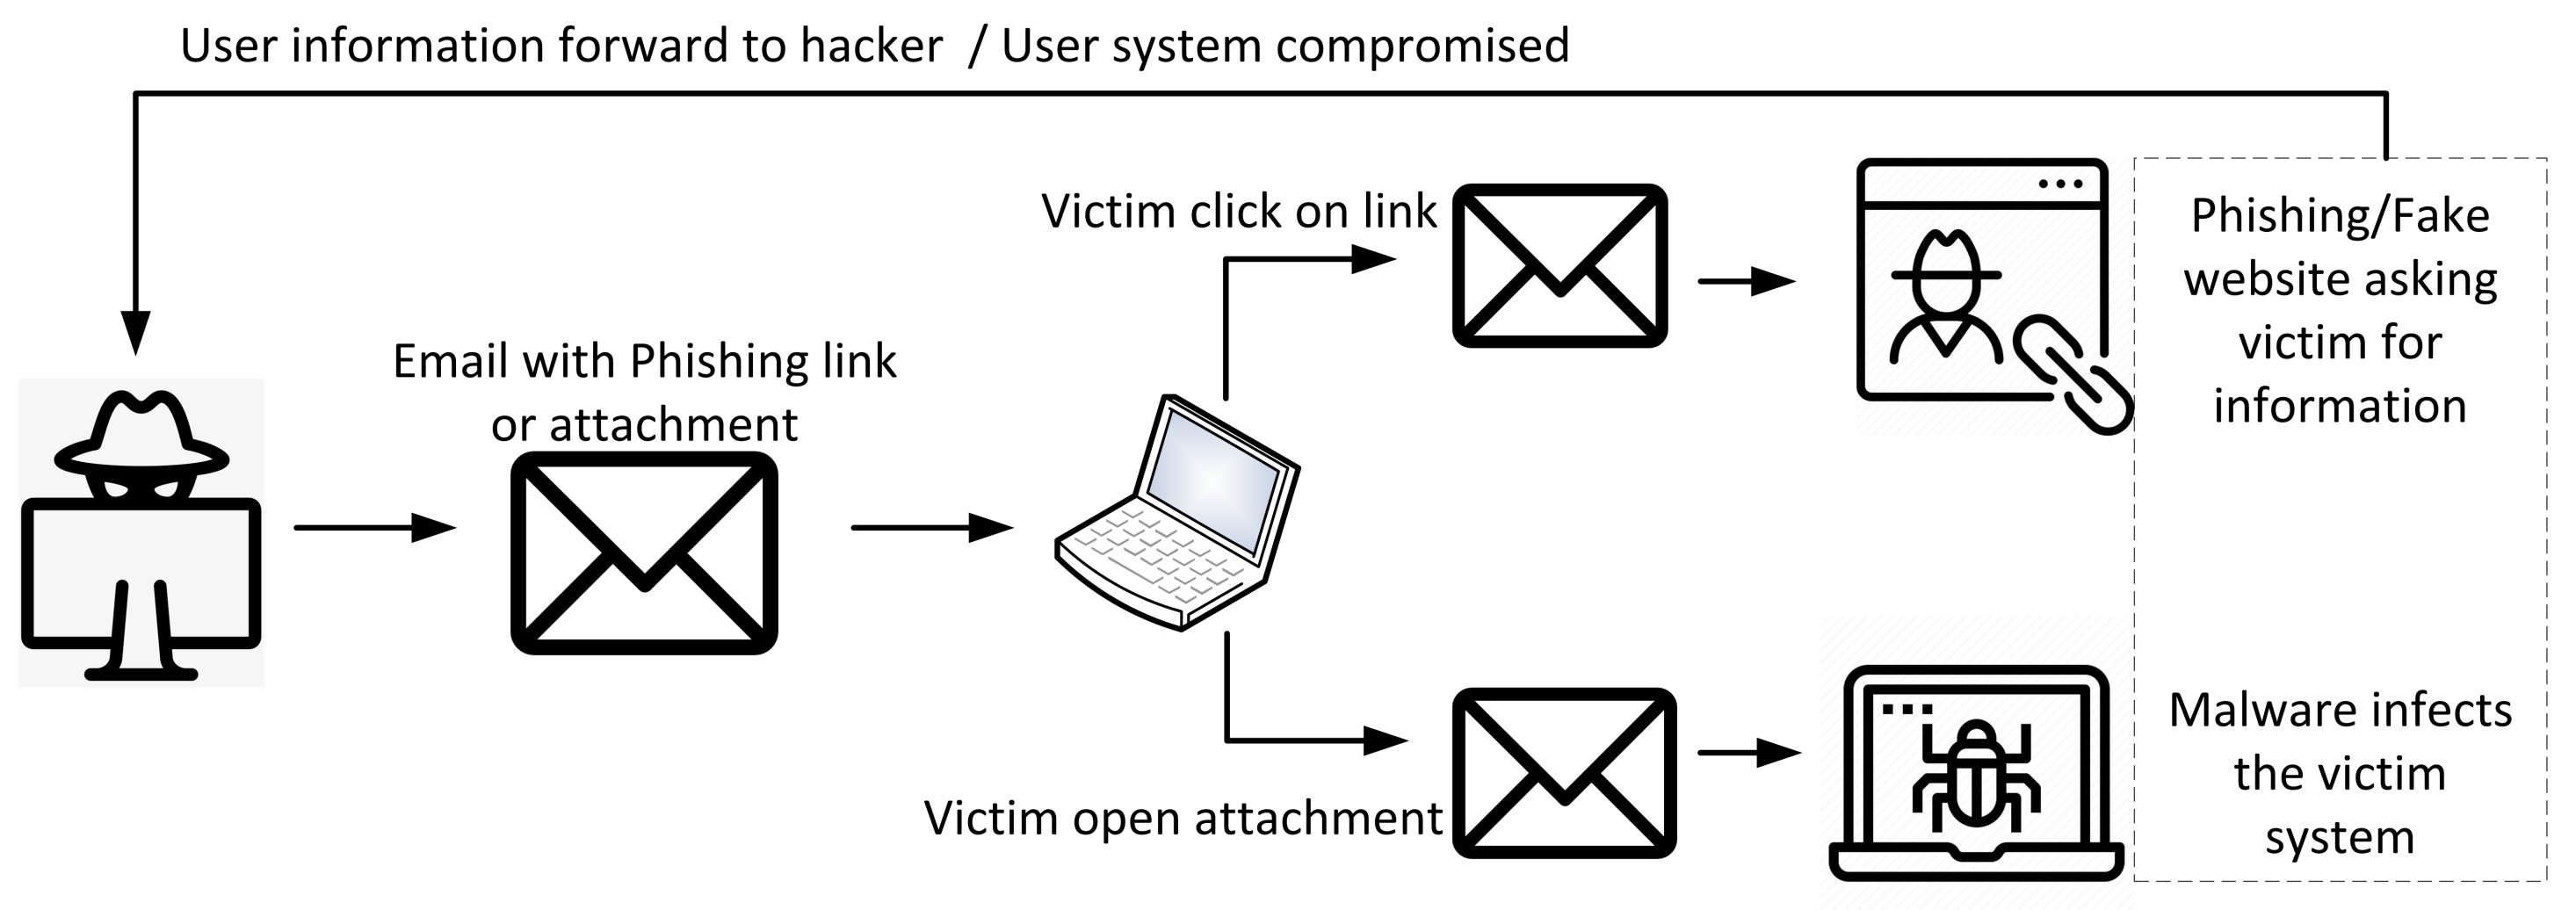
\includegraphics[width=1\linewidth]{phish.png}
    \caption{\textbf{FIGURE 2. }Common phishing attack workflow}
    \label{fig:placeholder}
\end{figure}
\subsubsection{Table 2. Common Types of Phishing Attacks}


\begin{table}
    \centering
    \begin{tabular}{cc}
         Phishing Attack& Description\\
         Spear& A spearphishing attack is a highly targeted, personalized scam designed to trick specific individuals or organizations into revealing sensitive information. Unlike a generic phishing attempt that casts a wide net, Spearphishers meticulously research their targets to craft convincing emails hat appear to come from a trusted source, such as a colleague, vendor, or executive.\\
         Whaling& A whaling attack is a highly targeted form of phishing that specifically goes after high-level executives and key decision-makers within an organization. Like hunting a "big fish," attackers focus on these "whales" because of their authority and access to valuable data and significant funds. The goal is to manipulate them into revealing sensitive information or transferring large sums of money to fraudulent accounts.\\
         Vishing& Vishing is a type of cybercrime in which attackers use deceptive phone calls and voicemail messages to manipulate individuals into disclosing sensitive personal information, such as bank account details, credit card numbers, Social Security numbers, or login credentials. It is essentially the "voice" version of phishing, where scammers typically impersonate representatives from trusted organizations, such as banks, government agencies (such as the IRS or Social Security Administration), tech support, or even family members.\\
         Smishing& Smishing is a form of cybercrime that uses deceptive text messages to trick individuals into giving up sensitive information, downloading malware, or sending money. The name is a blend of "SMS" (Short Message Service) and "phishing." Smishing attacks are effective because people tend to be less skeptical of text messages compared to emails and often respond to them with a great sense of urgency.\\
         Impersonation& An impersonation attack is a form of social engineering in which a cybercriminal pretends to be a known or trusted person or entity to deceive a victim. The attacker's goal is to manipulate the target into taking actions that benefit the criminal, such as transferring funds, sharing sensitive information, or revealing login credentials. Unlike malware-based attacks that exploit software vulnerabilities, impersonation attacks exploit human psychology and a person's natural tendency to trust. They can occur through various methods and means, both digital and physical.\\
         Business Email Compromise (BEC)& Business Email Compromise (BEC) is a sophisticated type of cybercrime where attackers use email to impersonate a trusted individual or organization, such as a CEO, vendor, or legal counsel, to trick employees into taking actions that benefit the attacker, such as wiring funds or sharing sensitive information.\\
         Clone Phishing& Clone phishing is a cyberattack where an attacker creates a nearly identical copy of a legitimate, previously-sent email to deceive recipients. By perfectly replicating the branding, language, and sender details, the attacker replaces original links or attachments with malicious ones. This tactic exploits a victim's trust in a familiar source, making the fraudulent email very difficult to detect.\\
         Social Media Phishing& Social media phishing is a cyberattack that uses social networking platforms to trick users into revealing sensitive information, such as passwords, credit card numbers, and other personal data. Threat actors create fake profiles, send malicious links, or hack legitimate accounts to deceive victims and exploit their trust in familiar platforms.\\
         Distributed Spam Distraction (DSD)& Distributed Spam Distraction (DSD) is a cyberattack in which a user's inbox is flooded with thousands of non-malicious emails to distract them from more serious criminal activities happening in the background. This deluge of spam, often from thousands of different senders, serves as a smokescreen to hide alerts about fraudulent purchases or account changes. The attack relies on the fact that a user's attention is limited. By overwhelming the inbox with junk email, attackers hope the victim will miss the few critical, legitimate-seeming emails from banks or other financial institutions reporting unauthorized activity.\\
    \end{tabular}
    \caption{Commonly social engineering attacks}
    \label{tab:placeholder}
\end{table}
\subsection{Dumpster Diving}
It is only appropriate to start out this section by reiterating the adage:
\begin{quote}
    One Man's Trash Is Another Man's Treasure
\end{quote}
Dumpster diving is essentially looking for treasure in someone else's trash. In the world of cybersecurity, dumpster diving is a technique used to retrieve information that could be used to carry out an attack or gain access to a computer network from carelessly disposed items.

Dumpster diving is a low-tech yet effective method used to gather information about a target by searching through discarded materials such as trash or recycling bins. Attackers look for documents, receipts, notes, or other items that may contain sensitive data-including passwords, payslips, bills, credit card details, PII, or internal organizational information such as intellectual property and proprietary information, or trade secrets.

Furthermore, dumpster diving is not limited to searching through the trash for obvious treasures, such as access codes or passwords written down on forgotten sticky notes. Seemingly innocent and innocuous information, such as an old contact list, calendar, or organizational chart, can be used to assist an attacker using social engineering tehcniques to gain access to the network. This method is also one of the most common tactics used in identity theft.

To prevent dumpster divers from learning anything valuable from trash, it is recommended to establish a secure disposal policy where all paper-including print-outs- are shredded in a cross-cut shredder before being recycled, all storage media is degaussed and all staff educated about the danger of untracked trash.

Disposed computer hardware, including printers which contain internal hard drives, can be a gold mine for attackers. Information can be easily recovered from storage media, including drives that have been imporoperly formatted or erased. This includes stored passwords and trusted certificates. Even without the storage media, the equipment may include \textit{Trusted Platform Module (TPM)} data or other hardware IDs that are trusted by an organization. An attacker may also be able to use the hardware to identify the equipment manufacturer to craft potential exploits if that hardware has any outstanding and undiscovered vulnerabilities.

\begin{figure}
    \centering
    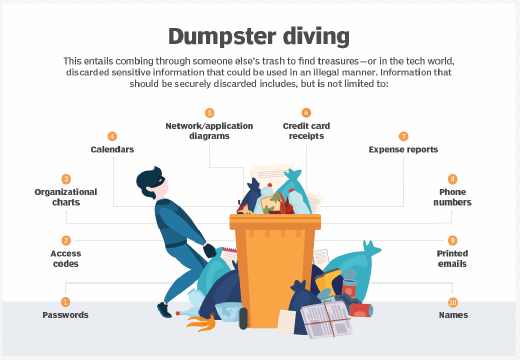
\includegraphics[width=0.75\linewidth]{dditems.png}
    \caption{\textbf{FIGURE 3. }Discarded items attackers can leverage in social engineering attacks via dumpster diving invasions}
    \label{fig:placeholder}
\end{figure}

Figure 3 illustrates the types of materials commonly found in organization's dumpster. These items are often carelessly disposed of without proper shredding, sanitization, or secure disposal, allowing malicious actors to retrieve and exploit the information for SE-based attacks.

\subsection{Dumpster Diving and Social Engineering Attacks Specifications}
Social engineering is using human interaction to trick another person into giving access or performing an action for the attacker. A primary goal of social engineering is to establish trust between the attacker and the target. Dumpster diving is a way for attackers to gain information that they use to establish trust and rapport, or a feeling of familiarity. While attackers will also take any computer equipment they find, the primary focus of a dumpster diving attack is to gain information about an organization and its inner-workings. Even innocuous documents can be used by an attacker for all the wrong reasons.

A list of names, such as a directory or phone list, can be used in many ways by an attacker. Employees' names can be used to guess their computer username, to attack their personal web accounts or for identity theft. A name list can also be used as part of a general phishing campaign against an organization or a spearphishing or whaling attack against an executive.

Telephone numbers can be used with Caller ID spoofing to coerce an employee to reveal other information in a voice phishing (vishing) attack. An attacker could use this to call an employee with a fabricated storyline such as, \textit{"Hi, this is Alyssa in accounting. The head of finance, Jayden, needs some numbers by tonight. I asked Damien, and he said to talk to you. Can you please help me?"}

Social engineering attacks use information gathered from dumpster diving. If attackers find a reciept for a vending machine restocking service, they may pretend to be employees of the service with a name badge on the same day and time as an expected delivery to gain access to areas that are otherwise never open to the public. Attackers could use this access to do a shoulder surfing or piggybacking attack or install a keylogger to gain access to the network in a passive manner.

\subsection{How to Prevent Dumpster Diving Attacks}
Although it may seem like a lot of work to properly care for trash, processes can be put in place to help prevent a dumpster diving attack. These should be documented and clearly explained to all employees and staff.

\textbf{Have a documented equipment decommissioning process.} Ensure all identifiable information is removed from computer equipment before it is disposed of or sold. This includes securely erasing data from hard drives, using burn bags to destroy paper evidence and clearing TPM data. Remove any trust factors in organizational databases , such as domain trust relationships, media access control (MAC) address authentication or expiring trust certificates.

\textbf{Use the appropriate secure storage media deletion process.} This may include securely erasing disk drives, shredding compact discs (CDs) and degaussing magnetic storage.

\textbf{Have a data retention policy, and use certificates of destruction for sensitive data.} Data retention policies should state how long documents and data should be kept and how they should be discarded. A certificate of destruction should be created and filed for legal tracking.

\textbf{Making shredding convenient.} Provide easy access to shredders next to recycling bins, or use secure shred bins next to every trash can. For employees who work from home, provide home paper shredders.

\textbf{Educate employees.} Provide information on proper disposal and typical social engineering methods. Do not allow employees to take printouts home, and do not give old computer equipment to employees.

\textbf{Secure trash.} Use locked trash and recycling bins, or keep refuse in a secure area until it is ready to be picked up. Use trusted equipment recyclers.

\begin{figure}
    \centering
    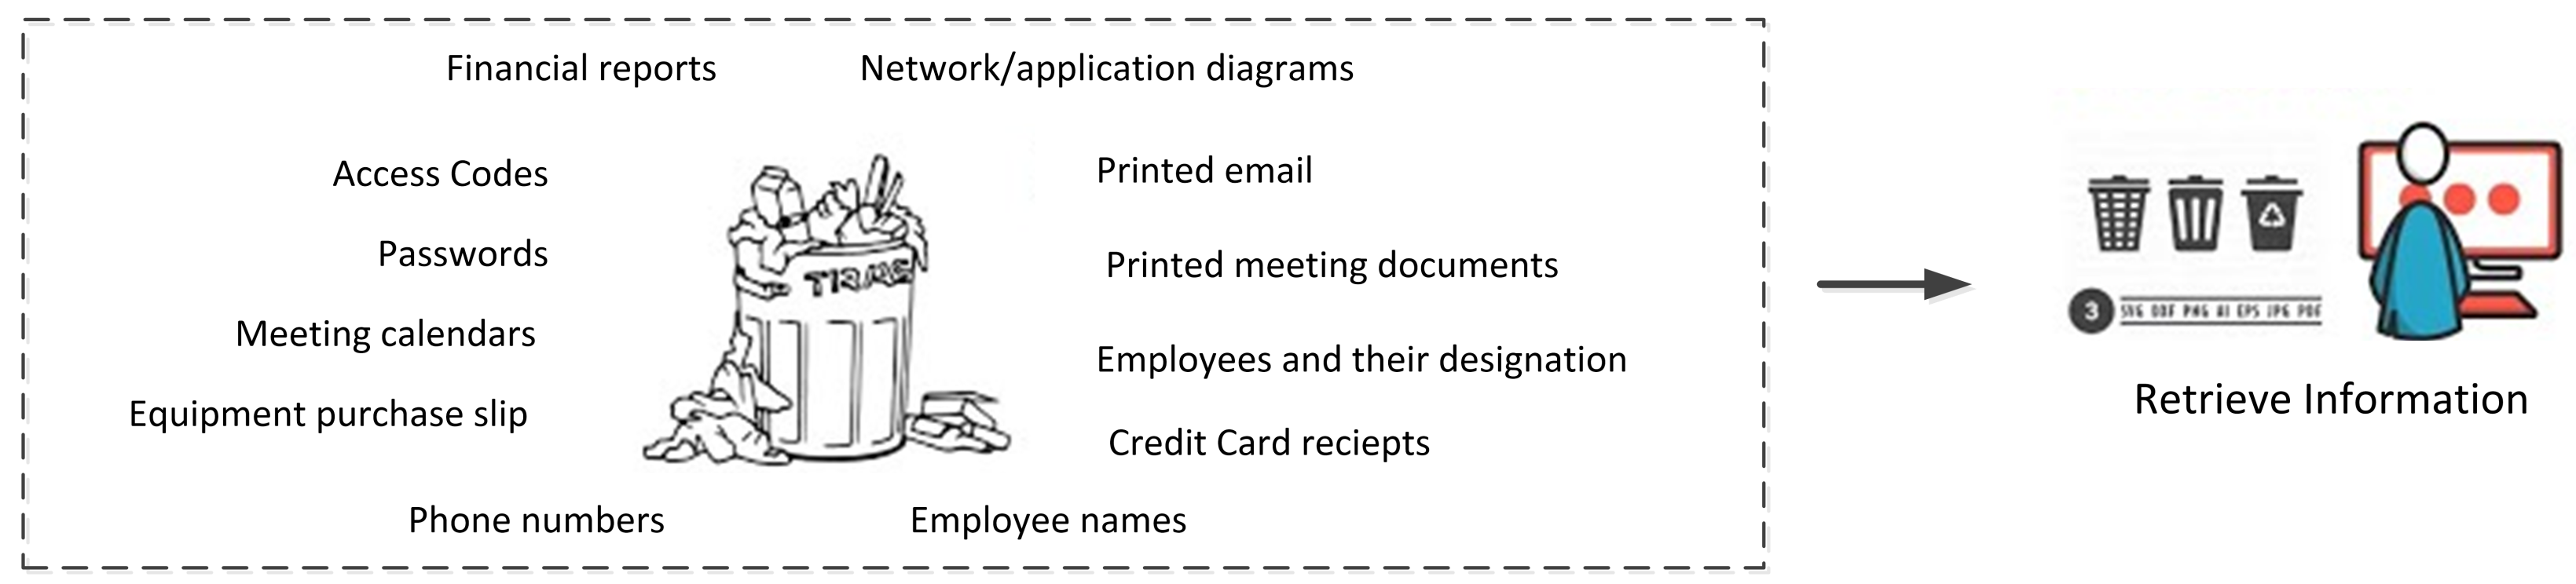
\includegraphics[width=0.75\linewidth]{dumpsterdive.png}
    \caption{Enter Caption}
    \label{fig:placeholder}
\end{figure}

\section{Scareware}
Scareware is a deceptive form of social engineering (SE) attack that exploits human psychology, aprticularly emotions such as fear, anxiety, urgency, and uncertainty, to coerce individuals into performing unsafe and many times, unethical actions. This type pf attack manipulates users by presenting alarming or fabricated warnings-typically in the form of pop-ups, fake alerts, or system notifications-intended to provide a quick, irrational response. The end goal is usually to trick the user into downloadinjg and installing malicious software, often under the guise of antivirus or system optimization tools.

The typical scareware attack begins with a strategically crafted message or alert that appears while the target is browsing the internet. As illustrated in Figure X, attackers often use malicious advertisements or compromised websites to display these pop-up warnings. These alerts commonly mimic legitimate security software (such as Windows, being the most popular one, with Amazon, and Best Buy in second and third), claiming that the system is infected with multiple "hard-drive destroying viruses" or that suspicious activity has been detected from your computer's IP address. To heighten hacking the human psychological impact, these warning often include alarming language ("Critical Threat Detected!" "You Lose All Data If Scan Is Not Run," "Your System is at Risk!") and visual elements such as flashing icons, faux scan results or security dashboards showing scores and percentages vulnerabilities identified on your compromised system, countdown timers, banners with the 1-800 number continually streaming across the page, and system logos that closely resemble trusted vendors like Micsoroft, Norton, McAfee, or Avast. Newer versions, and these ones hold true to the term "scareware" have an alert/alarm .wav so the alarm goes off as if it is D-Day, instilling irrational fear to move and act quickly within the target victim.

Once the victim clicks on the alert-typical out of panic or confusion-the attack escalates. The next step often involves presenting misinformation, such as false virus reports or system errors, accompanied by a proposed solution: downloading a supposed security tool or purchasing a fake antivirus license. In reality, this "solution" is either outright malware or software designed to harvest senstive information such as login credentials, financial data, and the like. In some cases, the scareware itself will act as ransomware, locking files and demanding payment for return.

The key to scareware's effectiveness lies in its manipulation of cognitive and emotional aspects and inherent vulnerabilities. It relies not on exploiting technical flaws in systems, but rather on exploiting the user's lack of technical knowledge and awareness and their instinct to protect their system from perceived threats. Because of this, even technically secure systems can be compromised if the user is successfully manipulated to bypass security controls.

Graphical design plays a critical role in the effectiveness of scareware. Attackers invest significant effort into replicating the look and feel of legitimate software interfaces. Common tactics include using the same color schemes or brand identifiers, layout structures, font styles, and logos as widely known antivirus vendors. This visual mimicry reinforces the illusion of legitimacy and trustworthiness, another great example of a deception tactic at work with increasing likelihood that the victim will comply with the attacker's demands.

Scareware represents a dangerous intersection of psychological manipulation and technical deception.  Demonstrates how adversaries can leverage user behavior, patterns, tells, and emotions to bypass even robust security measures.

\subsection{Countermeasures Against Scareware}
Effective defense against scareware requires a combination of technical controls-such as browser security settings, anti-malvertising tools, and real-time antivirus and malware monitoring-and user education aimed at raising awareness of these manipulative tactics.


\begin{figure}
    \centering
    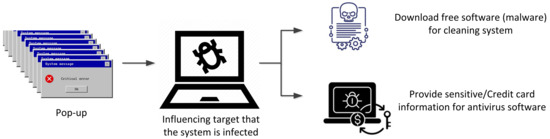
\includegraphics[width=1\linewidth]{scareware.png}
    \caption{\textbf{FIGURE 4. }Steps of a scareware attack}
    \label{fig:placeholder}
\end{figure}

\section{Water Hole}
A Water Hole Attack, also known as a watering hole attack or \textit{strategic website compromise}, is a sophisticated form of social engineering and \textit{supply chain attack} in which adversaries compromise legitimate websites that are known to be frequently visited by users within a specific target organization or sector. This method of attack draws its name from a predator's strategy in nature: just as animals gather at watering holes in the wild, where predators lie in wait, attackers in the digital world "lie in wait" at carefully selected websites to ambush unsuspecting users. This tactic has grown in popularity due to its stealth, effectiveness, and ability to target well-defended environments without directly attacking them.

Figure X provides a high-level overview of the multi-stage process that typically defines a water hole attack.


\begin{figure}
    \centering
    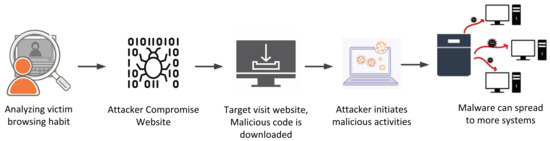
\includegraphics[width=0.75\linewidth]{waterhole.png}
    \caption{\textbf{FIGURE 5. }Steps of a water hole attack}
    \label{fig:placeholder}
\end{figure}

\subsubsection{\paragraph{\textbf{Step 1: Target Identification and Reconnaissance}}}
The first stage involves the reconnaissance of the target organization. The attacker selects an organization or industry based on strategic motivations—such as corporate espionage, geopolitical interests, or financial gain. Using open-source intelligence (OSINT) methods, attackers collect data about the organization’s infrastructure, key personnel, and common user behaviors.

Surveys, phishing campaigns, and traffic analysis are used to identify which websites are commonly accessed by employees. These may include third-party vendor portals, local government services, industry forums, supply chain partner websites, or even internal blogs and news sources. By identifying these “trusted” websites, attackers increase the likelihood of a successful compromise.

\subsubsection{\textbf{Step 2: Website Compromise}}
Once a frequently visited website is selected, the attacker attempts to compromise its infrastructure. This is often done through:

\begin{itemize}
    \item \textbf{Exploiting known CMS vulnerabilities} (e.g., WordPress plugins, outdated Joomla installations),
    \item \textbf{Phishing the site administrators}, or
    \item \textbf{Injecting malicious scripts} through third-party ad services or analytics.
\end{itemize}

The website may remain fully functional while silently delivering malware-laden scripts to its visitors. In recent cases, attackers have also used drive-by downloads or JavaScript-based malware that executes in the browser to profile users in real time.

\subsubsection{\textbf{Step 3: Profiling the Victim}}
When a victim visits the compromised site, malicious scripts run silently in the background to fingerprint the device. This step involves:

\begin{itemize}
    \item Inspecting the user-agent string to determine browser version and operating system,
    \item Collecting IP address and geolocation data,
    \item Checking installed browser plugins and extensions, and
    \item Running JavaScript or WebAssembly probes to detect vulnerabilities.
\end{itemize}

Some advanced attackers may even deploy \textbf{zero-day exploits} that specifically target vulnerabilities associated with software common in the environment of the target organization.

\subsubsection{\textbf{Step 4: Exploitation and Payload Delivery}}
Based on the profile results, a customized exploit is launched to compromise the victim’s machine. This can involve:

\begin{itemize}
    \item Remote code execution vulnerabilities,
    \item Privilege escalation tools, or
    \item Malware dropper mechanisms.
\end{itemize}

Once access is gained, the attacker installs a \textbf{persistent payload}, which may include \textbf{\textit{Remote Access Trojans (RATs)}},\textit{keyloggers}, or {network discovery tools}. These tools allow lateral movement within the network, privilege escalation, data exfiltration, or even ransomware deployment, depending on the attacker’s objective.

\subsection{\textbf{Real-World Examples and Current Relevance}}
Water hole attacks have been increasingly used in \textbf{Advanced Persistent Threat (APT)} campaigns. For example:
\begin{itemize}
    \item In 2017, \textbf{APT10 (a Chinese state-sponsored group)} carried out watering hole attacks on multiple aerospace and defense contractor sites to steal proprietary technologies.
    \item In 2021, \textbf{SolarMarker malware campaigns} used Google SEO poisoning to redirect users to compromised web pages designed as watering holes to install info-stealing malware.
    \item In 2024, researchers observed that watering hole tactics are being used in \textbf{supply chain attacks} on \textit{Managed Service Providers (MSPs)} and \textbf{ open source package repositories} such as \texttt{PyPI} and \texttt{npm}, significantly widening the attack surface.
\end{itemize}

\subsection{\textbf{Implications and Mitigation}}
Water hole attacks are particularly dangerous because they target \textbf{trusted external websites}, bypassing traditional perimeter defenses. Since traffic originates from seemingly legitimate sources, it often goes unnoticed by intrusion detection systems (IDS) or endpoint protection platforms unless advanced \textbf{behavioral analysis} or \textbf{threat intelligence feeds} are integrated.

\textbf{Mitigation strategies include:}

\begin{itemize}
    \item Network segmentation and endpoint isolation,
    \item Restricting or monitoring access to third-party sites,
    \item Keeping browsers and plugins updated,
    \item Deploying advanced \textbf{web filtering and sandboxing}, and
    \item Educating employees to recognize anomalous website behavior or certificate warnings.
\end{itemize}

Furthermore, using zero-trust architectures, where every external interaction is verified regardless of origin, can help defend against watering hole techniques.

In sum, the water hole attack is a compelling example of how attackers leverage both psychological trust and technical compromise to penetrate otherwise well-secured environments. As employees continue to interact with a wide range of online resources in hybrid or remote work models, the threat posed by watering hole attacks continues to escalate - necessitating a combination of user vigilance, proactive threat hunting, and robust technical defenses to mitigate risk effectively.

\warningbox{\lipsum[4]}




\section{Section Heading}
Instead of simply listing headings of different levels we recommend to let every heading be followed by at least a short passage of text. Furtheron please use the \LaTeX\ automatism for all your cross-references and citations.


\subsection{Subsection Heading}

Instead of simply listing headings of different levels we recommend to let every heading be followed by at least a short passage of text. Further on please use the \LaTeX\ automatism for all your cross-references\index{cross-references} and citations\index{citations} as has already been described in Sect.~
\subsubsection{Subsubsection Heading}
Instead of simply listing headings of different levels we recommend to let every heading be followed by at least a short passage of text. Furtheron please use the \LaTeX\ automatism for all your cross-references and citations as has already been described in Sect., see also Fig.~\ref{fig:1}\footnote{If you copy text passages, figures, or tables from other works, you must obtain \textit{permission} from the copyright holder (usually the original publisher). Please enclose the signed permission with the manucript. The sources\index{permission to print} must be acknowledged either in the captions, as footnotes or in a separate section of the book.}

Please note that the first line of text that follows a heading is not indented, whereas the first lines of all subsequent paragraphs are.

references and citations citations as has already been described in Sect.

Please note that the first line of text that follows a heading is not indented, whereas the first lines of all subsequent paragraphs are.

\begin{svgraybox}
If you want to emphasize complete paragraphs of texts we recommend to use the newly defined Springer class option \verb|graybox| and the newly defined environment \verb|svgraybox|. This will produce a 15 percent screened box 'behind' your text.

If you want to emphasize complete paragraphs of texts we recommend to use the newly defined Springer class option and environment \verb|svgraybox|. This will produce a 15 percent screened box 'behind' your text.
\end{svgraybox}


\subsubsection{Subsubsection Heading}
Instead of simply listing headings of different levels we recommend to let every heading be followed by at least a short passage of text. Furtheron please use the \LaTeX\ automatism for all your cross-references and citations as has already been described in Sect.~\ref{ }.

Please note that the first line of text that follows a heading is not indented, whereas the first lines of all subsequent paragraphs are.

\begin{theorem}
Theorem text goes here.
\end{theorem}
%
% or
%
\begin{definition}
Definition text goes here.
\end{definition}

\begin{proof}
%\smartqed
Proof text goes here.
%\qed
\end{proof}

\paragraph{Paragraph Heading} %
Instead of simply listing headings of different levels we recommend to let every heading be followed by at 